% =====================================================================
%  PORTFOLIO SECTION: Self-Reconfigurable Soft Robotic Modules
%  Chase Quijano
%
%  One section of a larger portfolio. Compiles standalone with pdfLaTeX
%  (Overleaf-ready). To merge into your master document, copy everything
%  between the SECTION START / SECTION END markers and keep ./images/.
% =====================================================================
\documentclass[10pt,letterpaper]{article}

\usepackage[T1]{fontenc}
\usepackage[utf8]{inputenc}
\usepackage{lmodern}
\usepackage[letterpaper,margin=0.85in]{geometry}
\usepackage{graphicx}
\usepackage{enumitem}
\usepackage{booktabs}
\usepackage{tabularx}
\usepackage{microtype}
\usepackage{multicol}
\usepackage{needspace}

\setlist[itemize]{leftmargin=1.4em,itemsep=2pt,parsep=0pt,topsep=3pt}
\newcommand{\captiontext}[1]{\par\vspace{2pt}{\footnotesize\itshape\raggedright #1\par}}

\pagestyle{empty}
\setlength{\parindent}{0pt}
\setlength{\parskip}{5pt}

\begin{document}

%== SECTION START =====================================================

{\large\bfseries Self-Reconfigurable Soft Robotic Modules: Undergraduate Student Researcher}\\
Rowan University \,·\, May 2024 -- Present
\vspace{2pt}
\hrule
\vspace{4pt}

Self-reconfigurable soft robotic modules require compact, reliable, and
modular electronics to drive actuators, interface with sensors, and
communicate between units. The challenge is designing PCBs that integrate
seamlessly with soft robotic hardware under strict space and reliability
constraints, including the ability to maintain flexion during operation.
I own the module electronics: the custom flexible mainboards, the docking
and addressing architecture, and the on-board actuation drivers, now in
their fourth design iteration.

\begin{itemize}
  \item \textbf{Iterated four generations of custom flexible PCBs:}
        engineered to withstand extreme mechanical strain and high-angle
        bending without trace de-lamination.
  \item \textbf{Integrated dynamic I\textsuperscript{2}C multiplexing and
        structural addressing onto individual docking faces:} enabling
        interlocking actuator modules to autonomously discover and map
        neighboring orientation nodes.
  \item \textbf{Embedded localized motor drivers and transistor-driven
        solenoid arrays on-board:} managing autonomous module interlocking
        and soft-actuator inflation cycles, supporting one forthcoming
        co-authorship.
\end{itemize}

\subsection*{Design Constraints}

\begin{itemize}
  \item The board must fit inside each soft robotic module: a
        96\,$\times$\,28\,mm outline with mechanical keep-outs and a
        low-profile component height budget.
  \item Flexible PCB capable of maintaining roughly 1$^{\circ}$ of flexion
        for extended periods without trace failure.
  \item Actuator control and sensor input on-board, including a bend
        sensor for future positional data collection.
  \item Reliable power distribution and communication between modules.
  \item Two-layer layouts in KiCad to stay within the research budget,
        manufacturable with flexible PCB processes and assembled in the
        lab; low-profile SMD components throughout, with DRV8833 motor
        drivers selected for reliability, availability, and current
        capacity matched to the actuators.
\end{itemize}

\subsection*{Four Mainboard Generations}

The mainboard is now on its fourth iteration, and the progression is the
clearest record of my growth as an electronics designer. The first board
shipped with a few incorrect traces that had to be bridged with jumper
wires, and used through-hole transistors that fought the space
constraints. Each generation after that folded in the lessons of the
last: verifying every net through design review before fabrication,
moving fully to SMD to shrink the footprint and simplify assembly,
replacing discrete microcontroller interface pads with a compact 11-pin
FPC connector to a secondary microcontroller board, and consolidating the
routing for reliability under repeated flexion. Comparing the V1 and V4
layouts below shows how much the design matured: cleaner net
organization, deliberate component placement, and a board designed to be
manufactured and serviced, not just to work once.

\vspace{2pt}
\begin{center}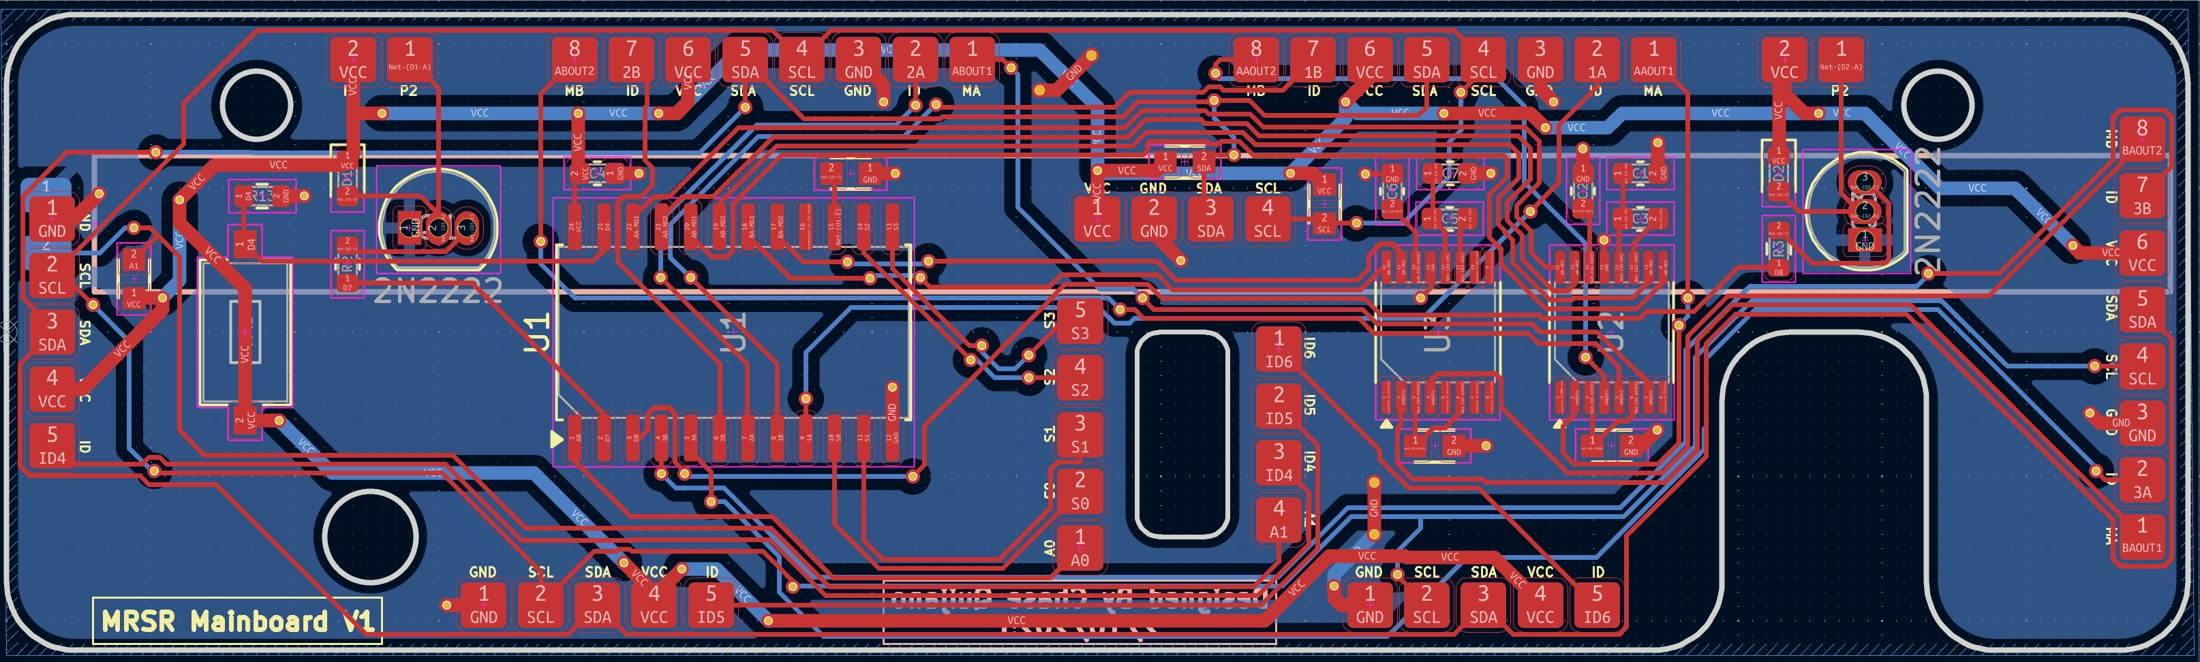
\includegraphics[width=0.93\textwidth]{images/layout_v1.jpg}\end{center}\vspace{-6pt}
\captiontext{Mainboard V1 layout: first-generation two-layer design with
through-hole transistors and discrete interface pads. This revision
required jumper-wire fixes after fabrication.}

\vspace{4pt}
\begin{center}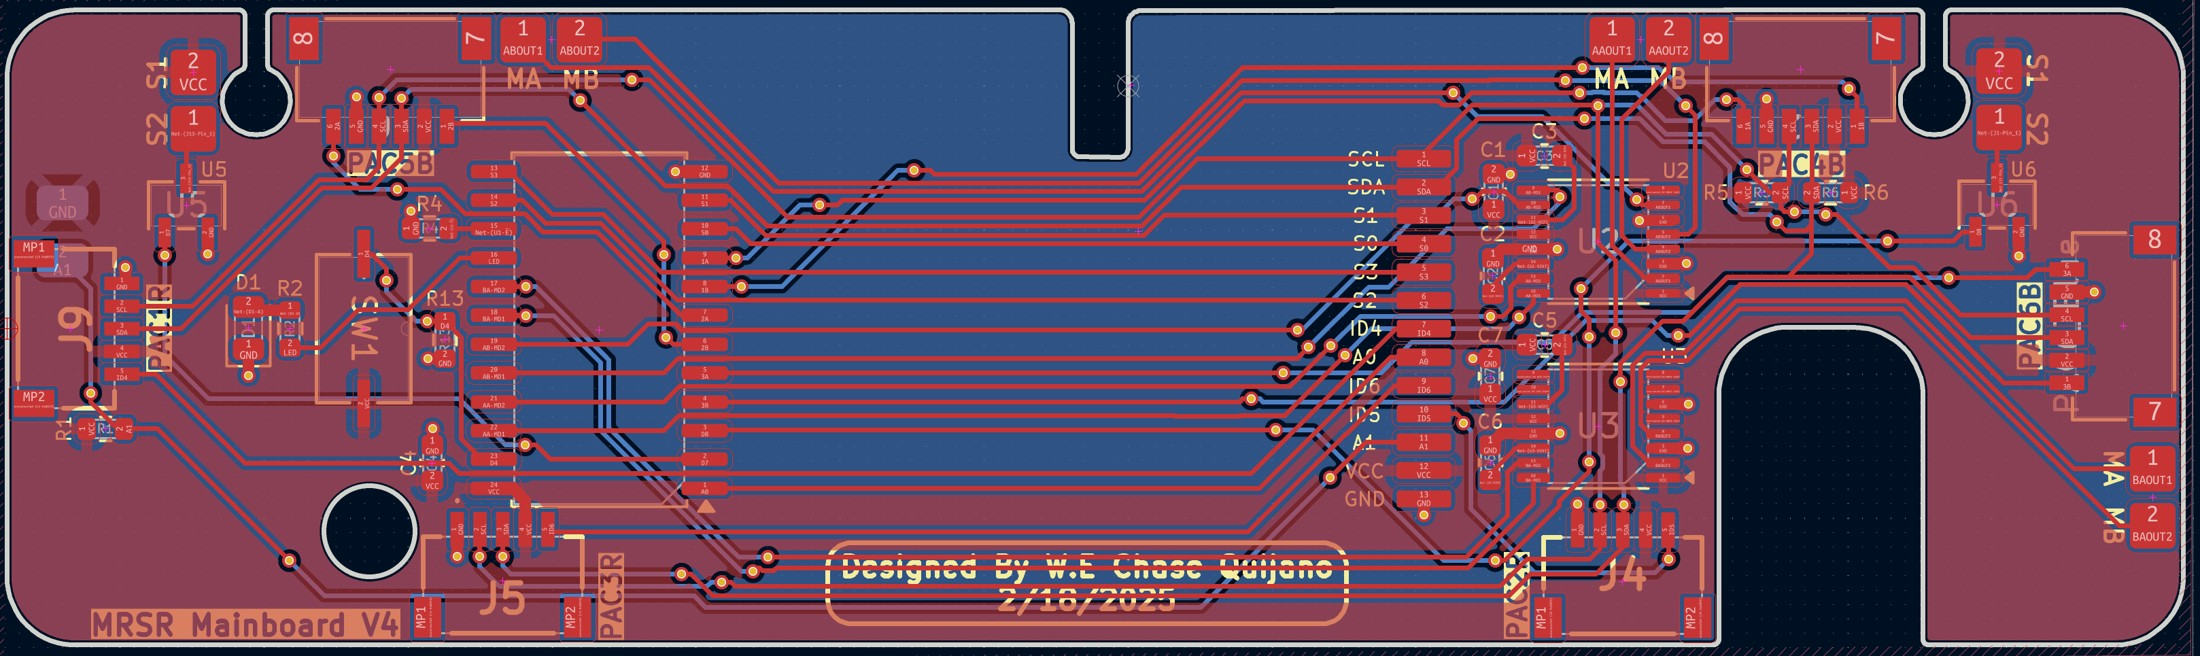
\includegraphics[width=0.93\textwidth]{images/layout_v4.jpg}\end{center}\vspace{-6pt}
\captiontext{Mainboard V4 layout: the latest iteration, fully SMD with
FPC interconnects, consolidated routing, and placement driven by the
module's mechanical and flexion constraints.}

\vspace{4pt}
\begin{minipage}[t]{0.435\textwidth}
  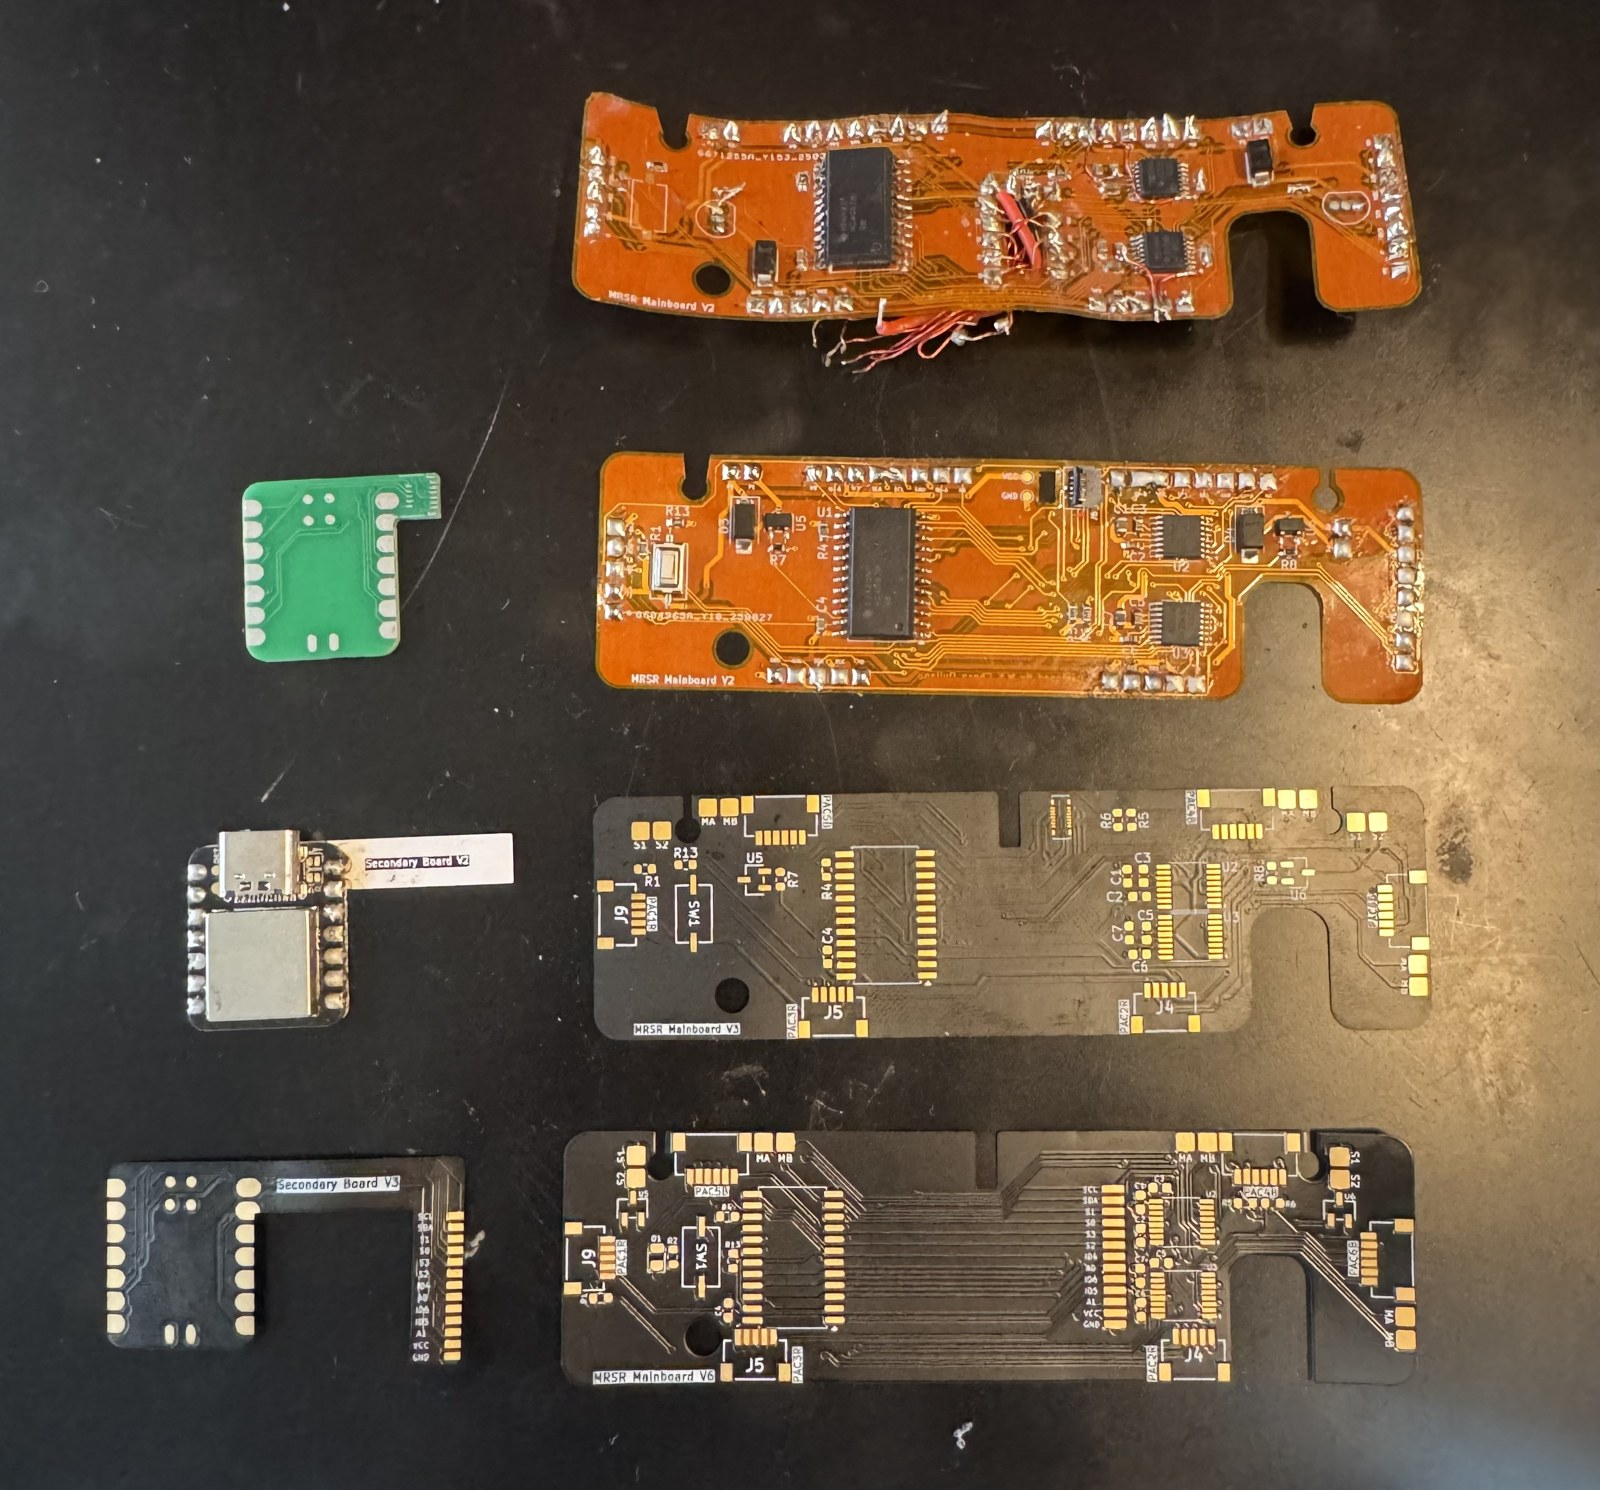
\includegraphics[width=\linewidth]{images/board_lineage.jpg}
  \captiontext{The mainboard lineage laid out: early flexible generations
  with hand-bodged fixes alongside the clean later revisions and their
  secondary microcontroller boards.}
\end{minipage}\hfill
\begin{minipage}[t]{0.435\textwidth}
  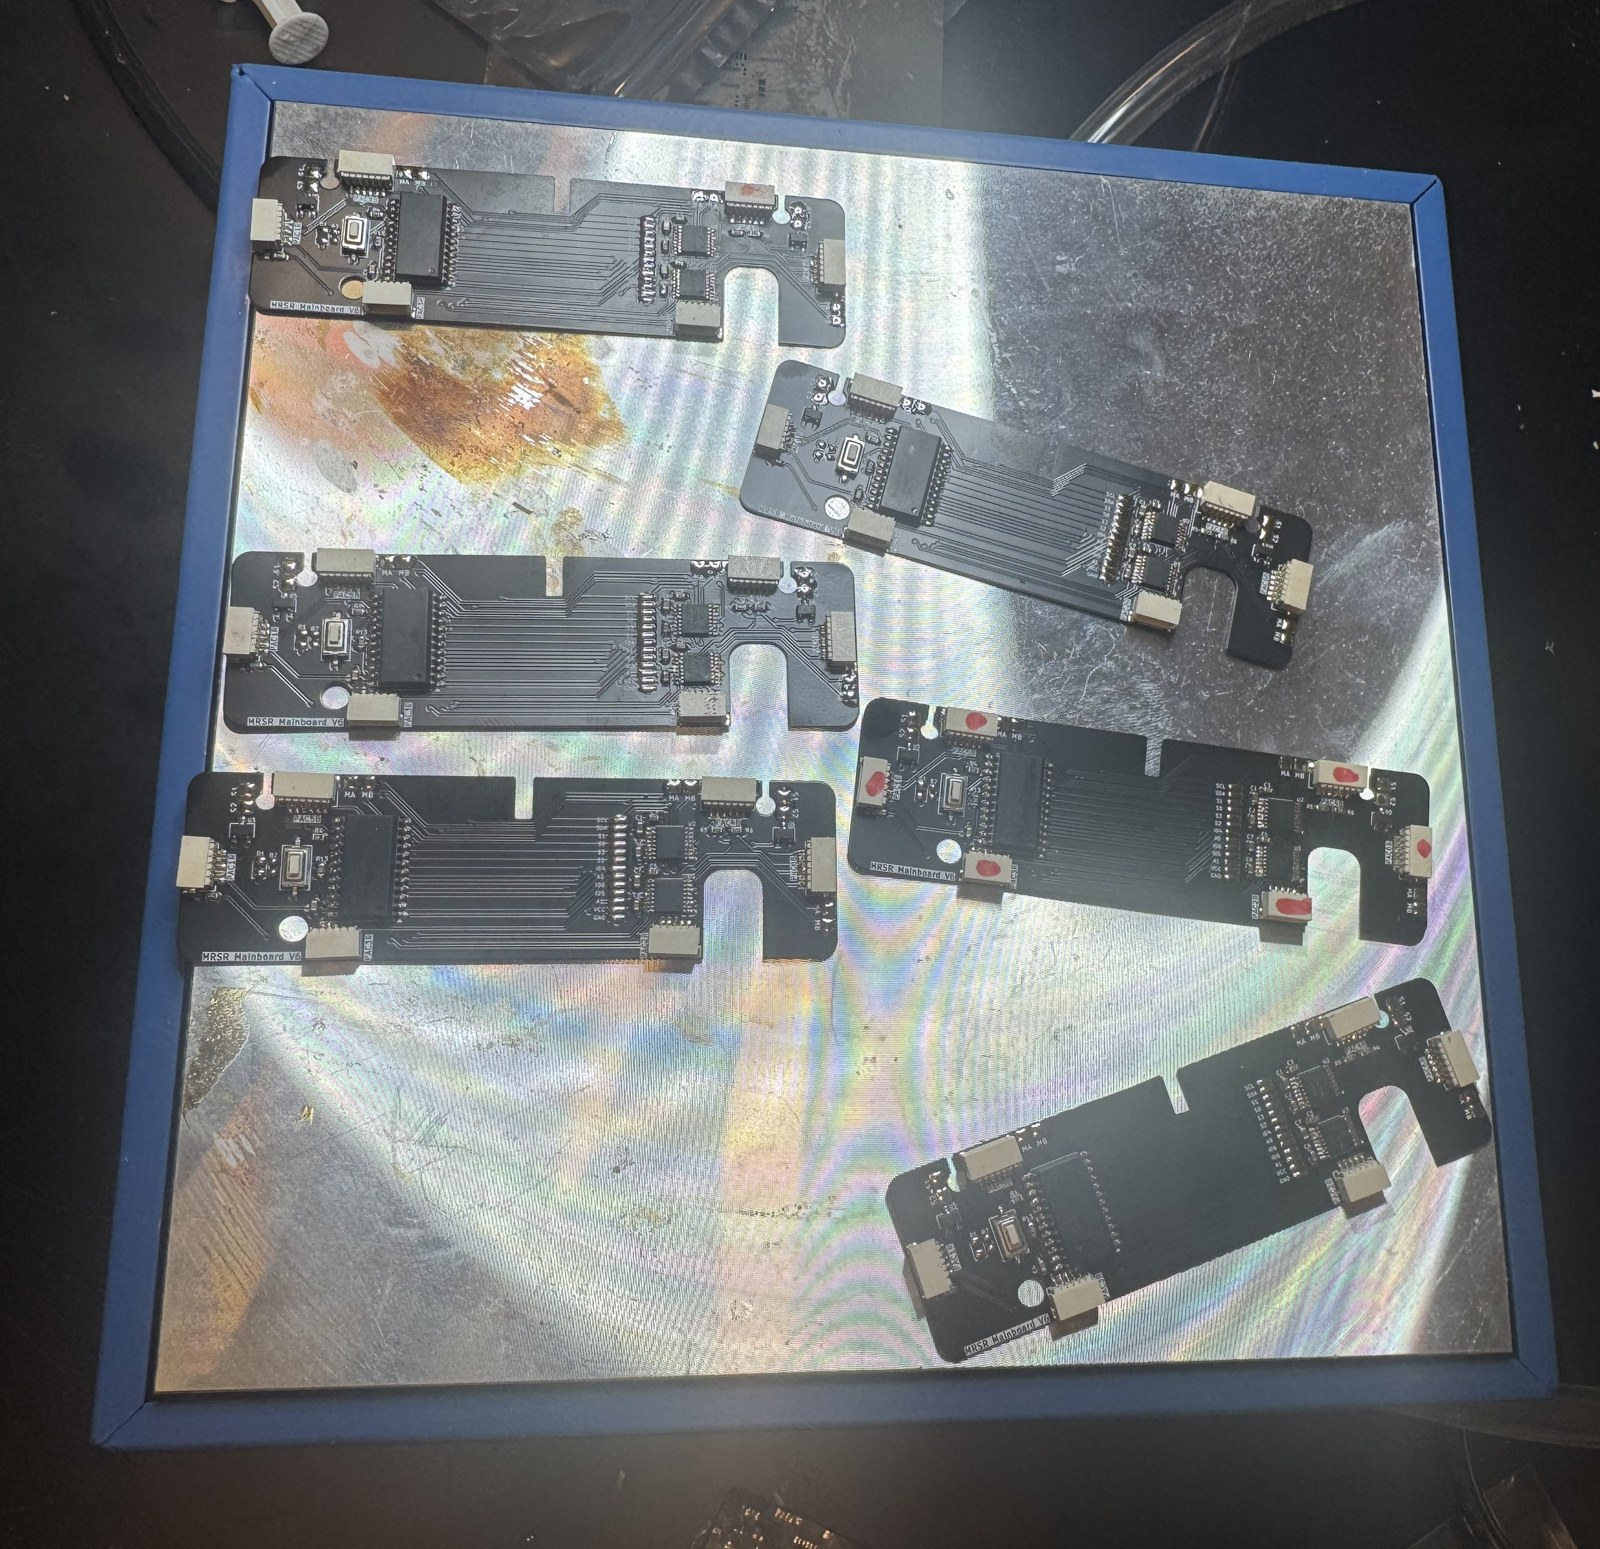
\includegraphics[width=\linewidth]{images/board_panel.jpg}
  \captiontext{A production run of the latest mainboard revision,
  hand-assembled and ready for module integration.}
\end{minipage}

\subsection*{Autonomous Docking and On-Board Actuation}

Each docking face carries its own addressing hardware: dynamic
I\textsuperscript{2}C multiplexing and structural addressing let a module
identify which neighbor is attached to which face and in what
orientation, so a chain of interlocked modules can autonomously discover
and map its own topology. The mainboard also embeds the actuation layer
locally, with motor drivers and transistor-driven solenoid arrays
managing the interlocking mechanisms and soft-actuator inflation cycles
without external drive electronics.

\vspace{2pt}
\begin{minipage}[t]{0.235\textwidth}
  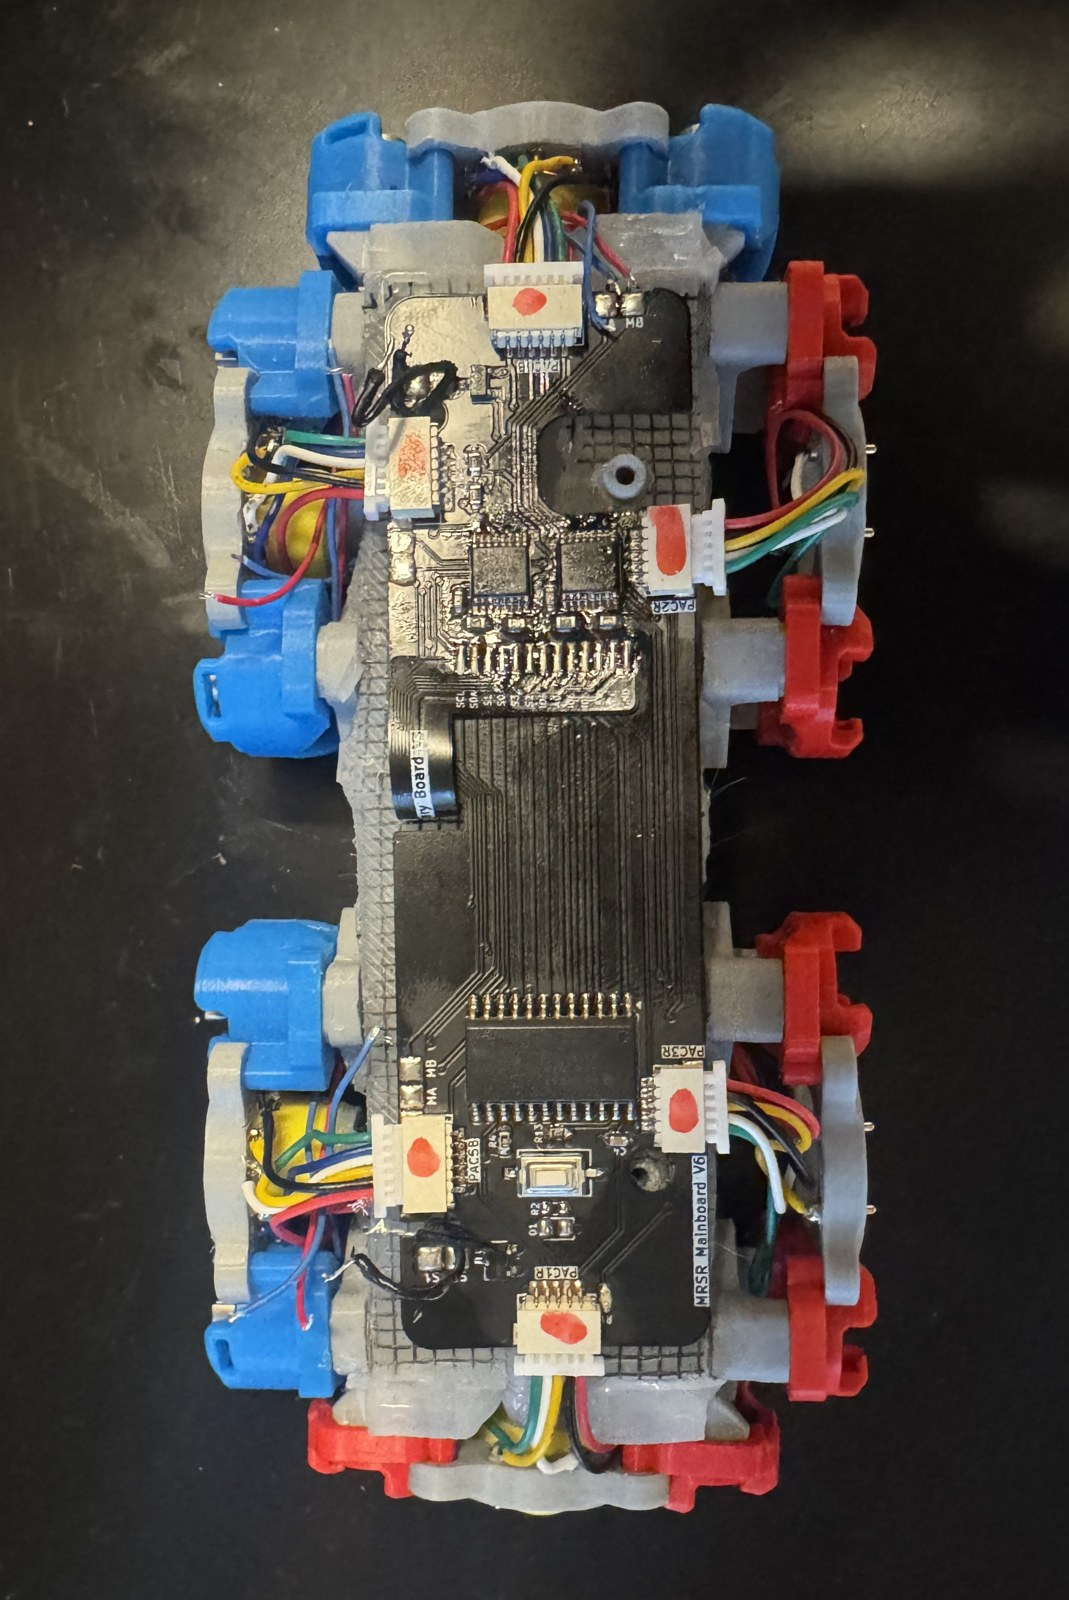
\includegraphics[width=\linewidth]{images/module_assembled.jpg}
  \captiontext{Assembled module with the latest mainboard installed:
  docking faces, PAC connectors, and actuation wiring integrated around
  the flexible board.}
\end{minipage}\hfill
\begin{minipage}[t]{0.47\textwidth}
  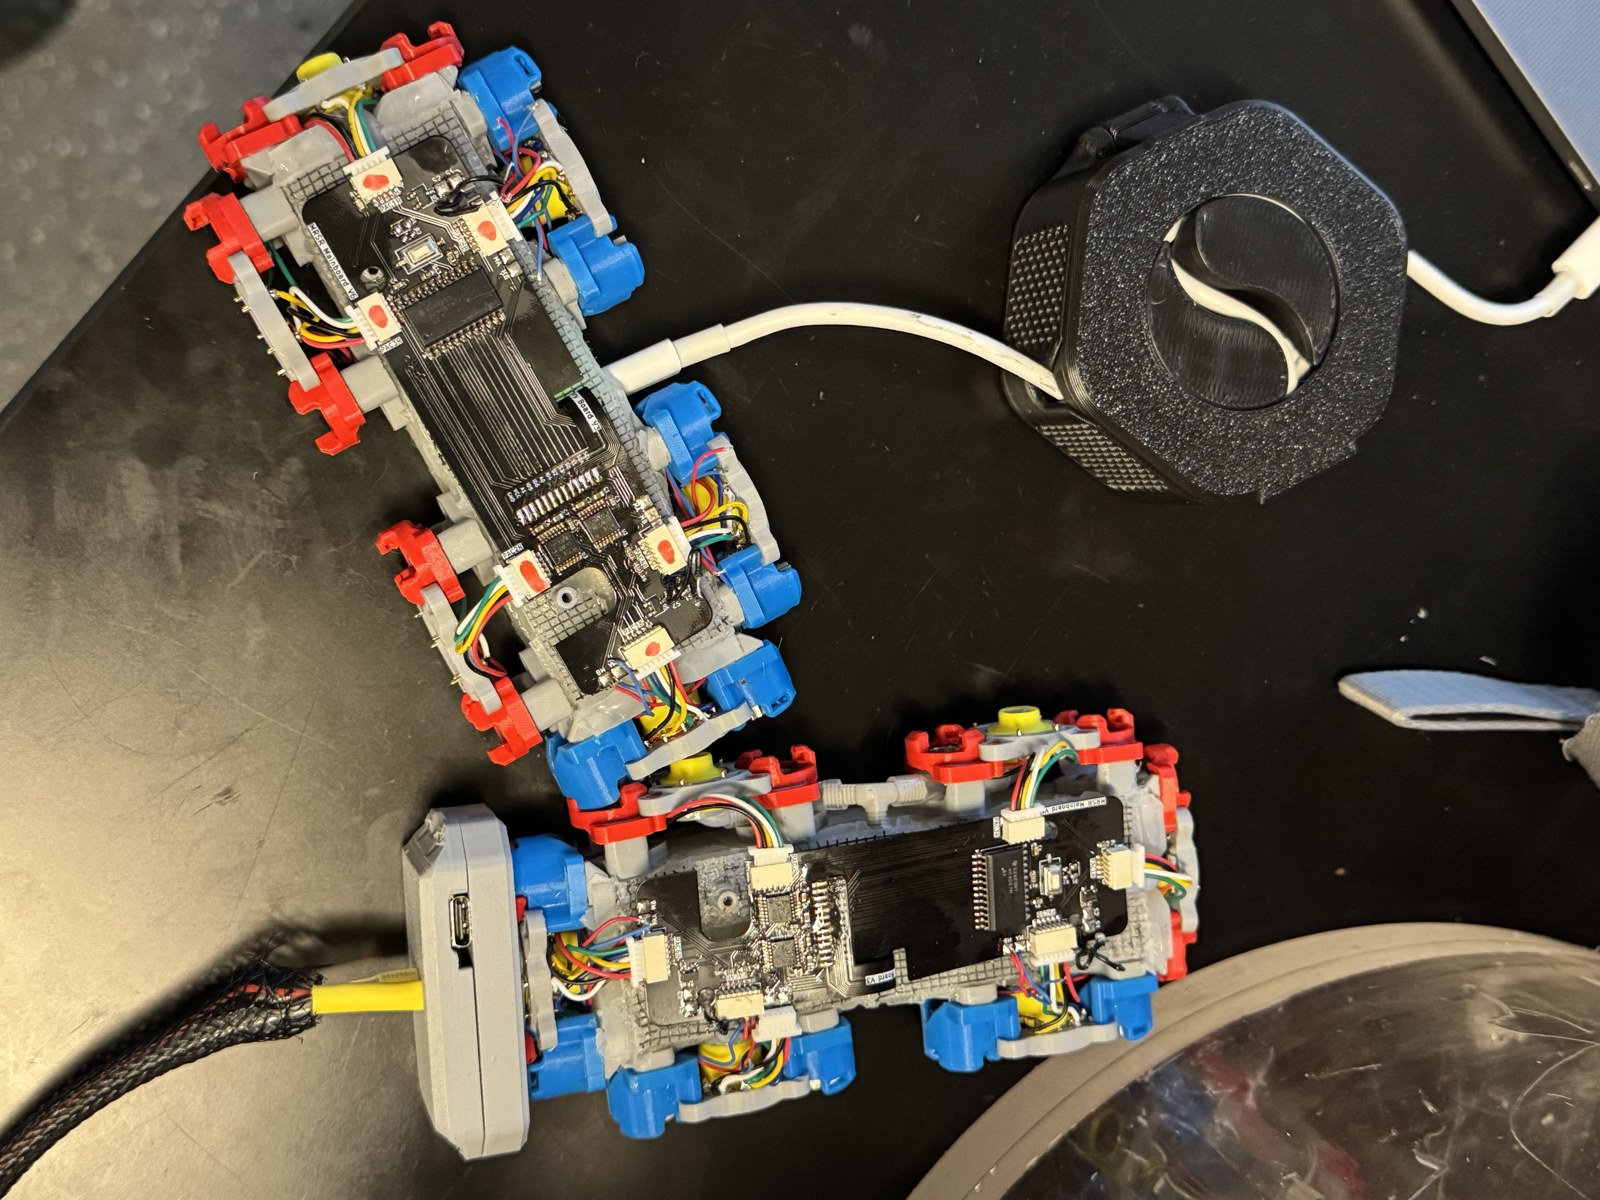
\includegraphics[width=\linewidth]{images/two_modules.jpg}
  \captiontext{Two modules interlocked and powered over USB during
  intermodule communication bring-up.}
\end{minipage}

\subsection*{Assembly, Testing, and Validation}

All boards are hand-assembled in the lab using SMT techniques (hot plate
and heat gun with solder paste) and inspected under a microscope for
solder joint integrity and trace bridging. Electrical validation
confirmed continuity and power integrity, and assembled modules have
successfully powered their actuators under load with stable performance,
including soft-actuator inflation testing. Extended flexion-cycle
reliability testing is planned in the upcoming research phase.

\vspace{2pt}
\begin{minipage}[t]{0.405\textwidth}
  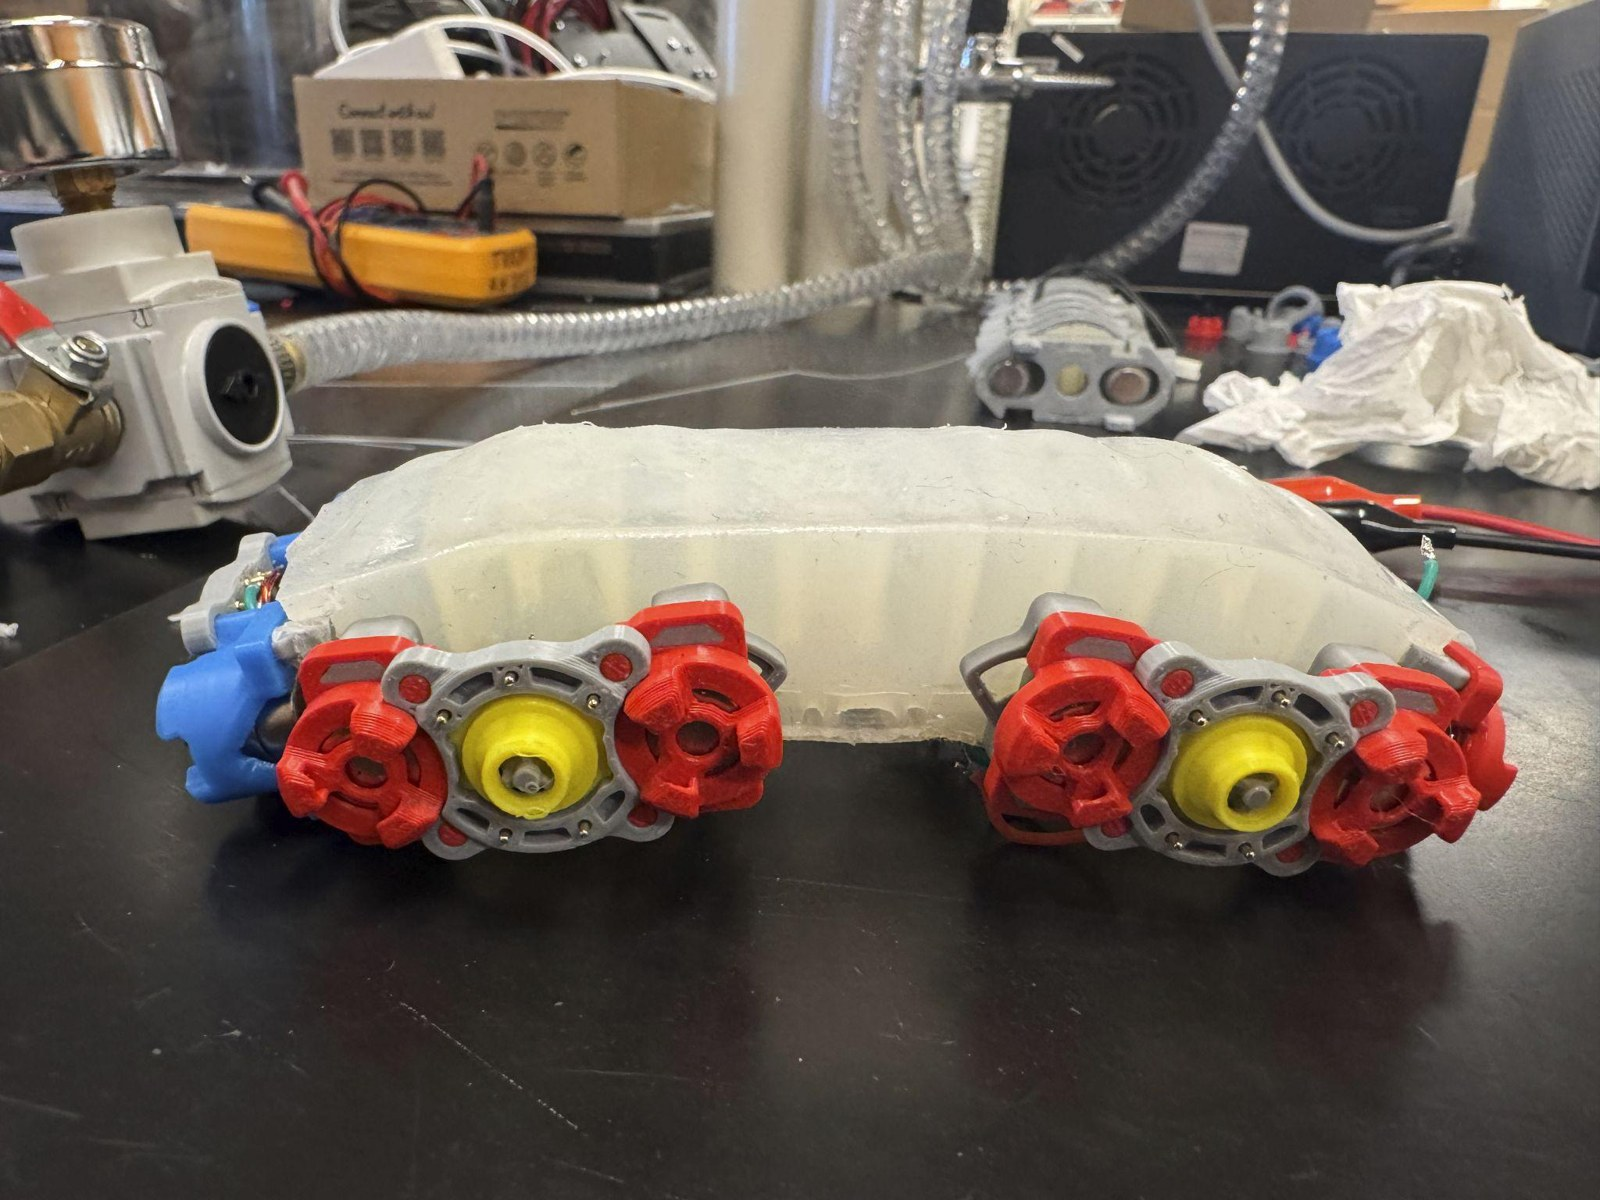
\includegraphics[width=\linewidth]{images/inflation_test.jpg}
  \captiontext{Module inflation test: the soft actuator pressurized with
  the docking hardware attached.}
\end{minipage}\hfill
\begin{minipage}[t]{0.405\textwidth}
  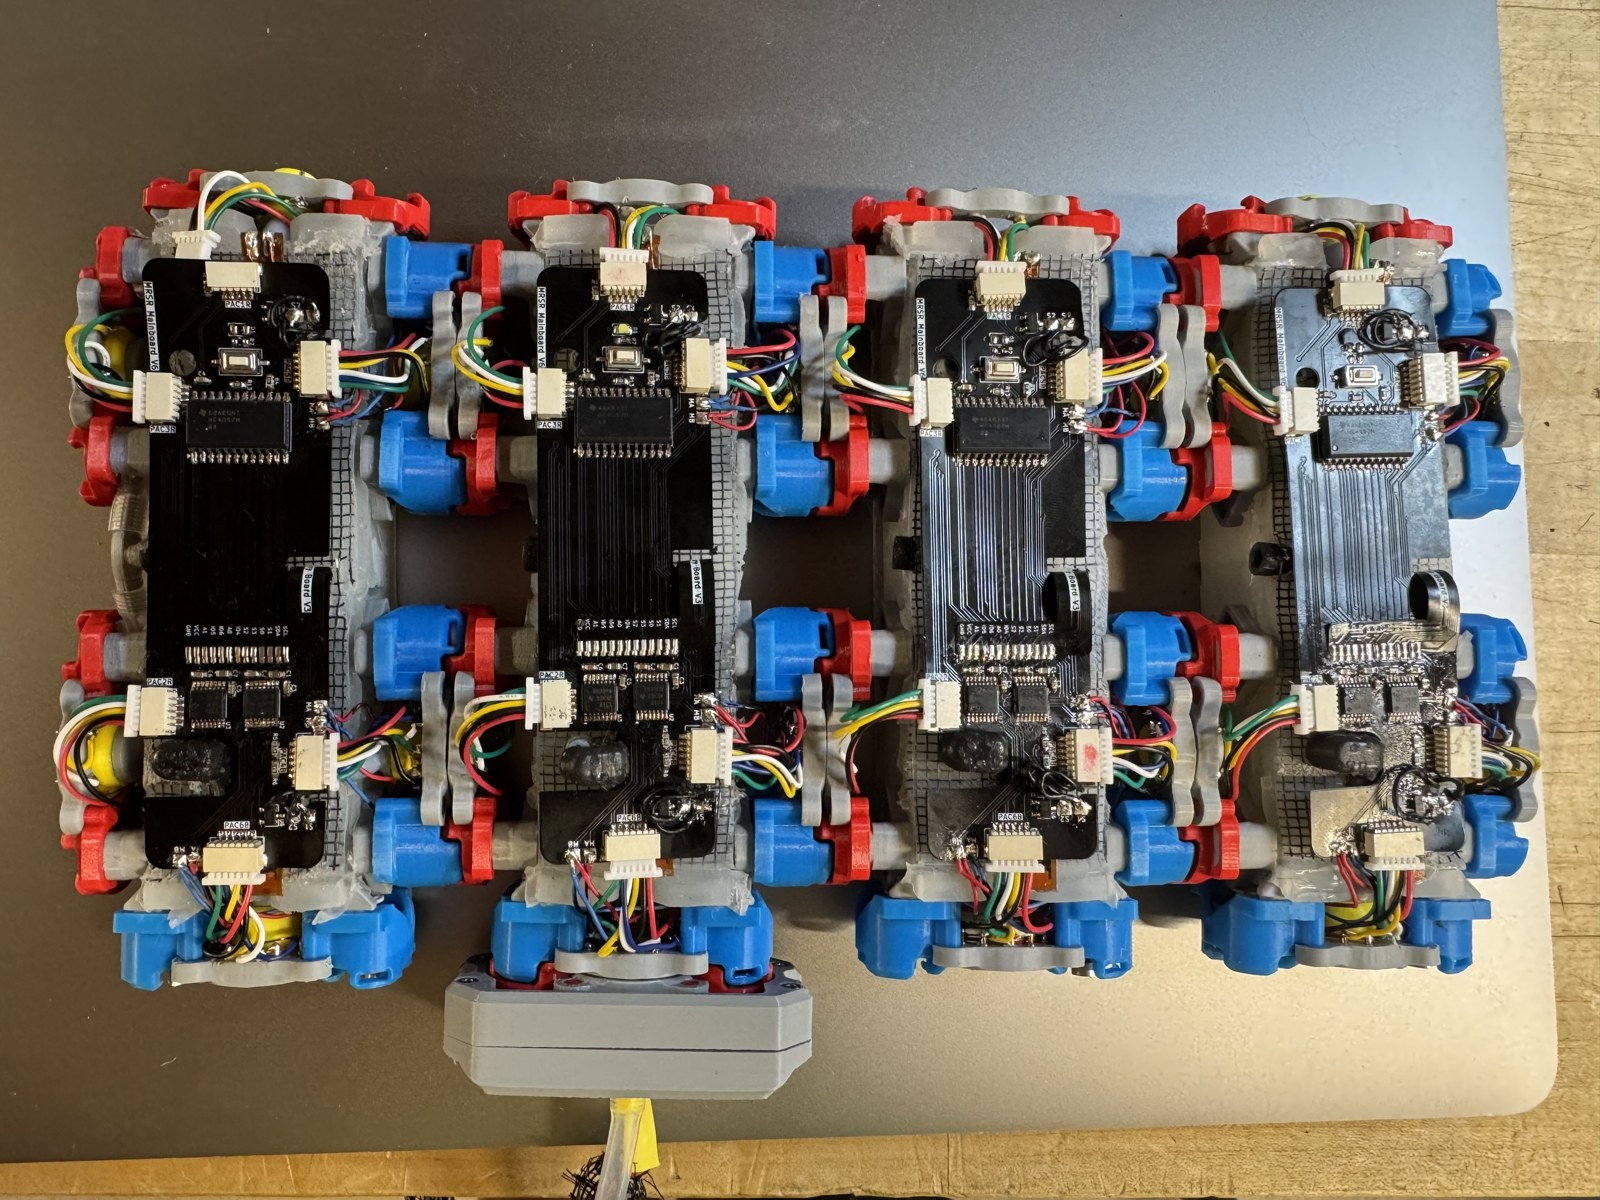
\includegraphics[width=\linewidth]{images/four_modules.jpg}
  \captiontext{Four modules with the latest mainboard revision installed,
  top-down view.}
\end{minipage}

\Needspace*{16\baselineskip}
\subsection*{Collaboration and Research Impact}

I work alongside graduate researcher Joshua Knospler to keep the PCB
form factor matched to the module mechanical design, and I assist in
module assembly and hardware refinements. The PCB systems described here
extend the group's published soft-robotics foundations by enabling more
compact, manufacturable, and modular electronics integration within the
modules. This contribution is included in a forthcoming publication on
which I am a co-author, and the research is currently being evaluated
for potential patenting and commercialization.

\vspace{4pt}
{\footnotesize
\textbf{Selected publications from this research group:}
\begin{enumerate}[leftmargin=1.6em,itemsep=1pt]
  \item J. Knospler, W. Xue, and M. Trkov, ``Reconfigurable modular soft
        robots with modulating stiffness and versatile task
        capabilities,'' \textit{Smart Materials and Structures}, vol.~33,
        no.~6, 2024.
  \item J. Knospler, N. Pagliocca, W. Xue, and M. Trkov, ``TendrilBot:
        Modular Soft Robot with Versatile Radial Grasping and Locomotion
        Capabilities,'' \textit{Sensors and Actuators A: Physical}, 2024.
  \item J. Knospler, W. Xue, and M. Trkov, ``MagBot: Reconfigurable
        Modular Soft Pneumatic Actuators with Tunable Magnetic Connection
        Mechanism,'' \textit{IEEE AIM}, 2024.
  \item J. Knospler, W. Xue, and M. Trkov, ``A Shared
        Electrical-Pneumatic and Reversible Locking Intermodule Connector
        for Modular Robots,'' \textit{IEEE AIM}, 2024.
  \item J. Knospler, N. Pagliocca, W. Xue, and M. Trkov, ``Realizing
        Modular Self-reconfiguring Soft Robots through Inter-module
        Communication and Model Checking,'' \textit{IEEE RoboSoft}, 2025.
\end{enumerate}}

%== SECTION END =======================================================

\end{document}
